\documentclass[english]{article}
\usepackage[T1]{fontenc}
\usepackage[utf8]{inputenc}
\usepackage{lmodern}
\usepackage[a4paper]{geometry}
\usepackage{babel}
\usepackage{fp}
\usepackage{pgf-pie}
\usepackage{hyperref}
\usepackage[section]{placeins}

% Define number image by symptom
\def \nbAlt {988}
\def \nbBig {665}
\def \nbMac {775}
\def \nbMil {894}
\def \nbMyc {772}
\def \nbPse {788}
\def \nbSym {890}

% Calculate number total of recto images
\FPadd\ttImgR\nbAlt\nbBig
\FPadd\ttImgR\ttImgR\nbMac
\FPadd\ttImgR\ttImgR\nbMil
\FPadd\ttImgR\ttImgR\nbMyc
\FPadd\ttImgR\ttImgR\nbPse
\FPadd\ttImgR\ttImgR\nbSym
\FPeval\ttImgR{round(ttImgR:0)}

% Calculate number total of images
\FPadd\ttImgRV\ttImgR\ttImgR
\FPeval\ttImgRV{round(ttImgRV:0)}

% Calculate proportion of each symptom
\FPdiv\pAlt\nbAlt\ttImgR
\FPmul\pAlt\pAlt{100}
\FPeval\pAlt{round(\pAlt:2)}
\FPdiv\pBig\nbBig\ttImgR
\FPmul\pBig\pBig{100}
\FPeval\pBig{round(\pBig:2)}
\FPdiv\pMac\nbMac\ttImgR
\FPmul\pMac\pMac{100}
\FPeval\pMac{round(\pMac:2)}
\FPdiv\pMil\nbMil\ttImgR
\FPmul\pMil\pMil{100}
\FPeval\pMil{round(\pMil:2)}
\FPdiv\pMyc\nbMyc\ttImgR
\FPmul\pMyc\pMyc{100}
\FPeval\pMyc{round(\pMyc:2)}
\FPdiv\pPse\nbPse\ttImgR
\FPmul\pPse\pPse{100}
\FPeval\pPse{round(\pPse:2)}
\FPdiv\pSym\nbSym\ttImgR
\FPmul\pSym\pSym{100}
\FPeval\pSym{round(\pSym:2)}

\title{Identification automatisée de multiples symptômes foliaires par vision numérique : apport des approches multi-vues}
\begin{document}

\maketitle

\tableofcontents

\section{Abstract}

\section{Materials and Method}

\subsection{General}
	\begin{figure}[!htbp]
		\includegraphics[scale=0.2]{images/ml_dl_process.png}
		\caption{workflow}
		\label{fig:workflow}
	\end{figure}
	\FloatBarrier
	
\subsection{Image database}
	The leaf’s shooting is standardized. We made a portable stand. (add photo) It composed of  a base  onto we fixed at left and right two LED light supports and at up a camera support. The LED lights are oriented to the middle of base.
	\\
	The image composition is standardized too. The background is uniform blue. At left, there is a ruler. At right, there are three color mire (black, gray and white). At down, we find photo’s name and orientation leaf (recto or verso). And at the middle, we put the leaf [\ref{fig:leaf_raw}].
	\begin{figure}[!htbp]
		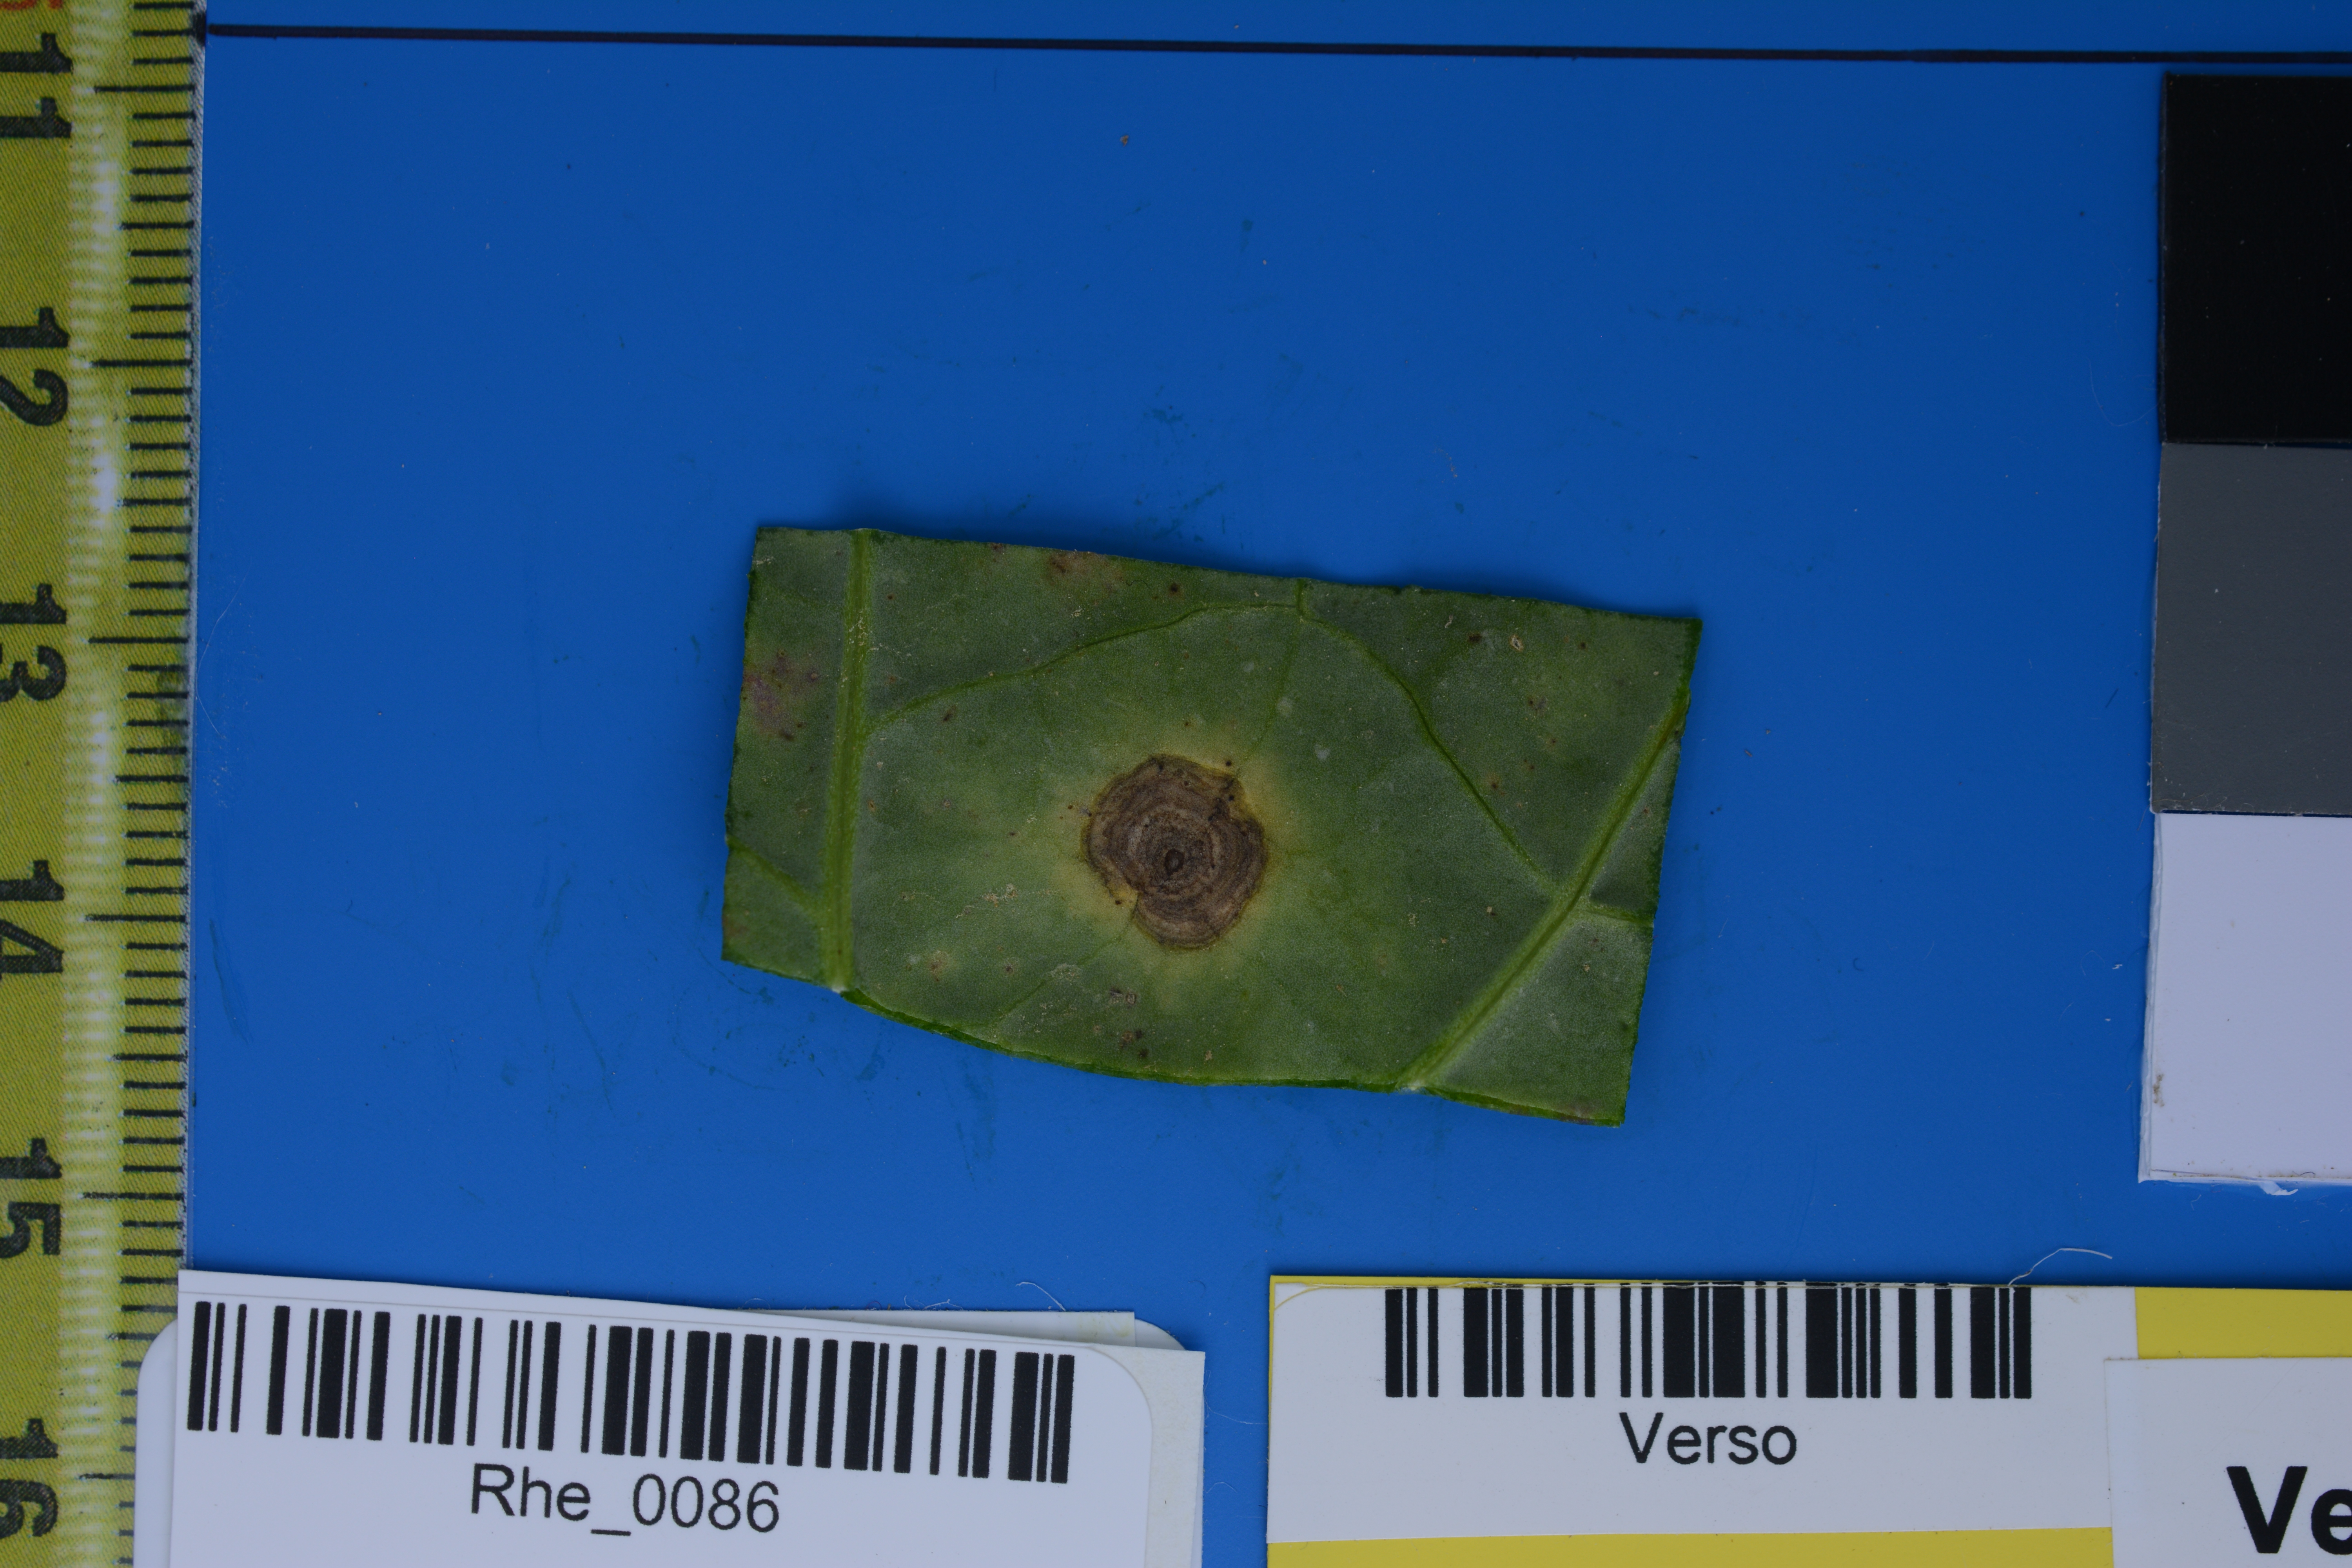
\includegraphics[scale=0.06]{images/leaf_raw.jpg}
		\caption{leaf raw}
		\label{fig:leaf_raw}
	\end{figure}
	\\
	In database, for each leaf we shoot the recto and the verso. A expert identify the symptom. Here we work on six symptoms, Alternaria (Alt), Biglobosa (Big), Maculense (Mac), Mildiou (Mil), Mycosephéréla (Myc), Pseudo (Pse) and symptom-less (Sym). We have \ttImgR leafs (so 9816 photos), \nbAlt Alternaria, \nbBig Biglobosa, \nbMac Maculence, \nbMil Mildiou, \nbMyc Mycosephéréla, \nbPse Pseudo and \nbSym Symptom-less [\ref{fig:Sym_dist}].

	\begin{figure}[!htbp]
		\begin{tikzpicture}
			\pie[
			text = legend
			]{\pAlt/Alt,
			  \pBig/Big,
			  \pMac/Mac,
			  \pMil/Mil,
			  \pMyc/Mic,
			  \pPse/Pse,
		      \pSym/Sym}
		\end{tikzpicture}
		\caption{Symptoms distribution}
		\label{fig:Sym_dist}
	\end{figure}
\end{document}
